\chapter{Anwendungsfall: Vermietung von Haushaltsgeräten nach dem Pay-as-You-Use Prinzip}
\label{ch:iot_usecase}
Qualitativ sehr hochwertige Haushaltsgeräte und Geräte für den professionellen Einsatz im Gastronomie-Umfeld haben hohe Anschaffungskosten, die der Privatanwender oder der Inhaber eines kleinen Gewerbes oftmals nicht leisten kann. Ein professioneller Kaffeevollautomat, eine leistungsfähige Spülmaschine oder eine Waschmaschine, die für hohe Kapazitäten ausgelegt ist, können Anschaffungskosten im vier bis fünfstelligen Euro-Bereich haben\footnote{Quelle!}. Eine naheliegende Möglichkeit besteht hier bei der Nutzung von Anbietern, die Haushaltsgeräte für eine monatliche oder jährliche Gebühr vermieten. So gibt es beispielsweise Anbieter für Kaffeemaschinen wie Tchibo\footnote{https://www.tchibo-coffeeservice.de/shop/kaffeevollautomaten/} oder Nespresso\footnote{https://www.nespresso.com/pro/de/de/kaffeemaschinen-buero}, die ihre Produkte direkt vermieten, oder Anbieter, die als Zwischenhändler fungieren und sich auf die Vermietung von Haushaltsgeräten verschiedener Hersteller spezialisiert haben. Dabei kommen klassische Miet- und Bezahlmodelle zum Einsatz, wobei es sich meistens um monatliche oder jährliche Mietgebühren handelt. Einen neuartigen Ansatz verfolgt das Unternehmen Winterhalter mit ihrem Pay-per-Wash\footnote{https://www.pay-per-wash.biz/ch\_de/} Ansatz. Hier bezahlt der Kunde keine monatliche Mietgebühr, sondern pro Waschgang; die Berechnung erfolgt also auf dem tatsächlichen Verbrauch des Kunden und nicht auf einer kalkulierten Pauschale.\\
Dieses Kapitel beschreibt einen IOT-Anwendungsfall, der die oben beschriebene Problematik aufgreift und das von der Firma Winterhalter eingeführte Pay-per-Wash Bezahlmodell einen Schritt weiterführt. Dabei interagieren verschiedene Stakeholder miteinander nach einem Pay-as-You-Use Prinzip auf einer einheitlichen Plattform.
%
% Section: Beschreibung
%
\section{Beschreibung}
\label{sec:iot_usecase:description}
Kunden mieten Haushaltsgeräte (im Consumer-Bereich oder für den professionellen Einsatz) wie Kaffeemaschinen oder Waschmaschinen je nach Anieter zum Nulltarif von verschiedenen Herstellern, die ihre Geräte auf einer Plattform zur Miete anbieten. Der genaue Verbrauch (Anzahl Kaffees, Menge an gewaschener Wäsche, Wasserverbrauch, etc.) wird mittels integrierter Sensoren an den Geräten erfasst und auf der Plattform persistiert. Damit wird ein genaues, vom tatsächlichen Verbrauch abhängiges Abrechnungsmodelle umgesetzt: Kunden zahlen nur das, was sie auch wirklich verbrauchen. Regelmäßige Reinigungen seitens der Kunden werden erfasst und durch ein entsprechendes Rabattmodell verrechnet. Serviceleistungen wie Wartung und Reparatur durch entsprechende Dienstleister können über die zugrundeliegende Plattform geplant, gesteuert und abgerechnet werden. Die Lieferung von Geräten, Ersatzteilen und Konsumgütern wie Kaffee oder Waschmittel erfolgt durch Lieferanten. Die Bestellung und Abrechnung wird über die zugrundeliegende Plattform koordiniert.\\
Die folgende Abbildung \ref{fig:chapter04:usecase} veranschaulicht den erläuterten Anwendungsfall.

\begin{figure}[htbp]
 \centering
 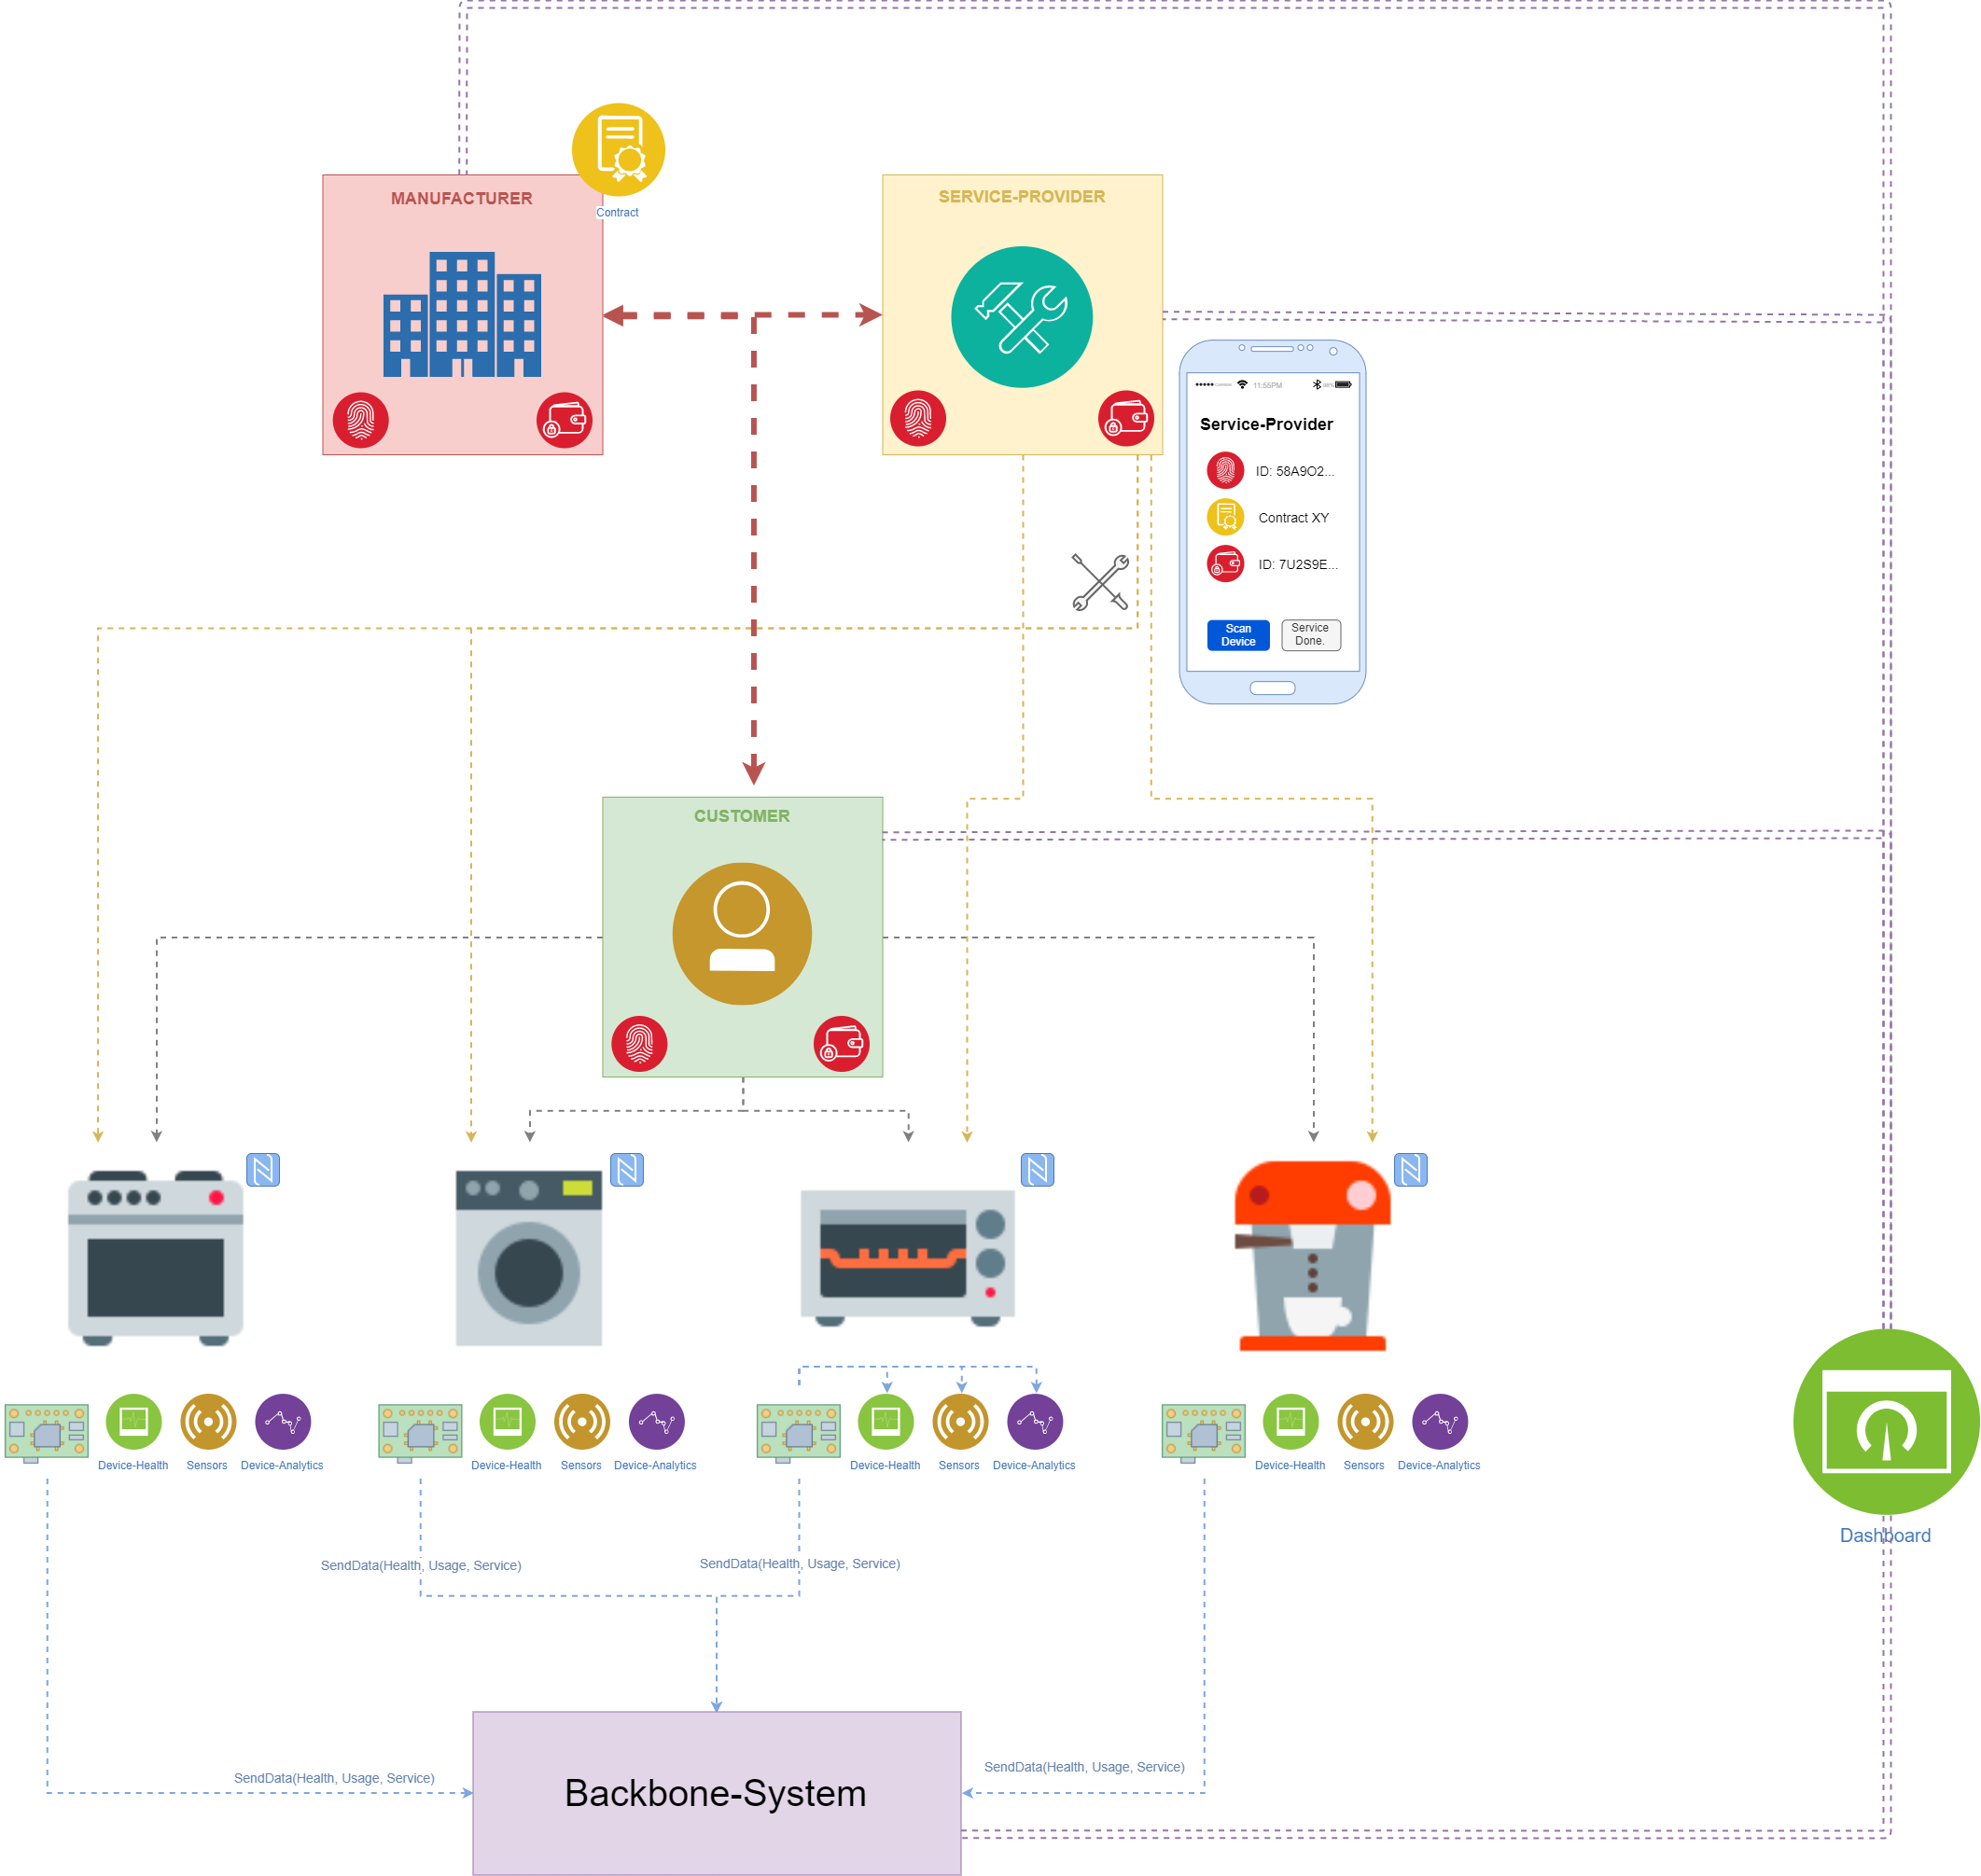
\includegraphics[width=1.0\textwidth]{gfx/IOT-Anwendungsfall.png}
 \caption{Grafische Veranschaulichung des Anwendungsfalls}
 \label{fig:chapter04:usecase}
\end{figure}


Der vorgestellte Anwendungsfall beinhaltet das Zusammenspiel mehrerer Stakeholder:
\begin{description}
\label{description:chapter04:stakeholder}
  \item[Hersteller] Der Hersteller der Geräte entwickelt und produziert die zu vermietenden Haushaltsgeräte und bietet diese zur Vermietung an Kunden auf der Plattform an. Er vertreibt Ersatzteile sowie Pflege- und Zusatzprodukte zu seinen Geräten, die Kunden und Service-Dienstleister erwerben können. Die vermieteten Geräte des Herstellers können Service-Dienstleister selbstständig und automatisiert für eine Reparatur oder eine Wartung beauftragen. Die Beauftragung und Abrechnung erfolgt über die Plattform. Für vermietete Geräte erhält der Hersteller nach einem Pay-as-You-Use Prinzip eine Bezahlung der Kunden entsprechend ihres Verbrauches.
  \item[Lieferant] Der Lieferant ist für die Lieferung der Geräte und Zusatzprodukte zu den Kunden und Service-Dienstleistern zuständig. Er holt die Ware beim Hersteller ab und liefert diese aus; die benötigten Adressinformationen sind auf der Plattform hinterlegt. Die Bezahlung für die Auslieferung erfolgt über die Plattform und berechnet sich automatisch über die Distanz der Lieferstrecke und der Abmessung der Ware.
  \item[Kunde] Der Kunde mietet Geräte vom Hersteller. Die Bestellung und Abrechnung erfolgt über die Plattform nach einem Pay-as-You-Use Prinzip. Die regelmäßige Reinigung der Geräte wird auf der Plattform protokolliert. Bei Einhaltung der vorgeschriebenen Reinigungsintervalle erhält der Kunde eine vertraglich festgelegte Gutschrift, bei Nicht-Beachten eine entsprechende Gebühr.  Darüber hinaus kann der Kunde auf Wunsch Konsumgüter wie Kaffee und Reinigungsmittel über die Plattform bestellen; dies geschieht vollautomatisch über das Gerät: Sobald die Menge des Produktes ein gewisses Limit unterschreitet, beauftragt das Gerät selbstständig den Kauf und die Anlieferung der Produkte über die Plattform.
  \item[Service-Dienstleister] Der Service-Dienstleister ist zuständig für die Wartung und Reparatur der Geräte und wird von den Geräten über die Plattform beauftragt.
\end{description}

Die Abbildung \ref{fig:chapter04:usecase_workflow} zeigt den groben Ablauf beginnend mit der Mietanfrage eines Kunden bis zur monatlichen Bezahlung der Teilnehmer für ihre Leistungen.

\begin{figure}[htbp]
 \centering
 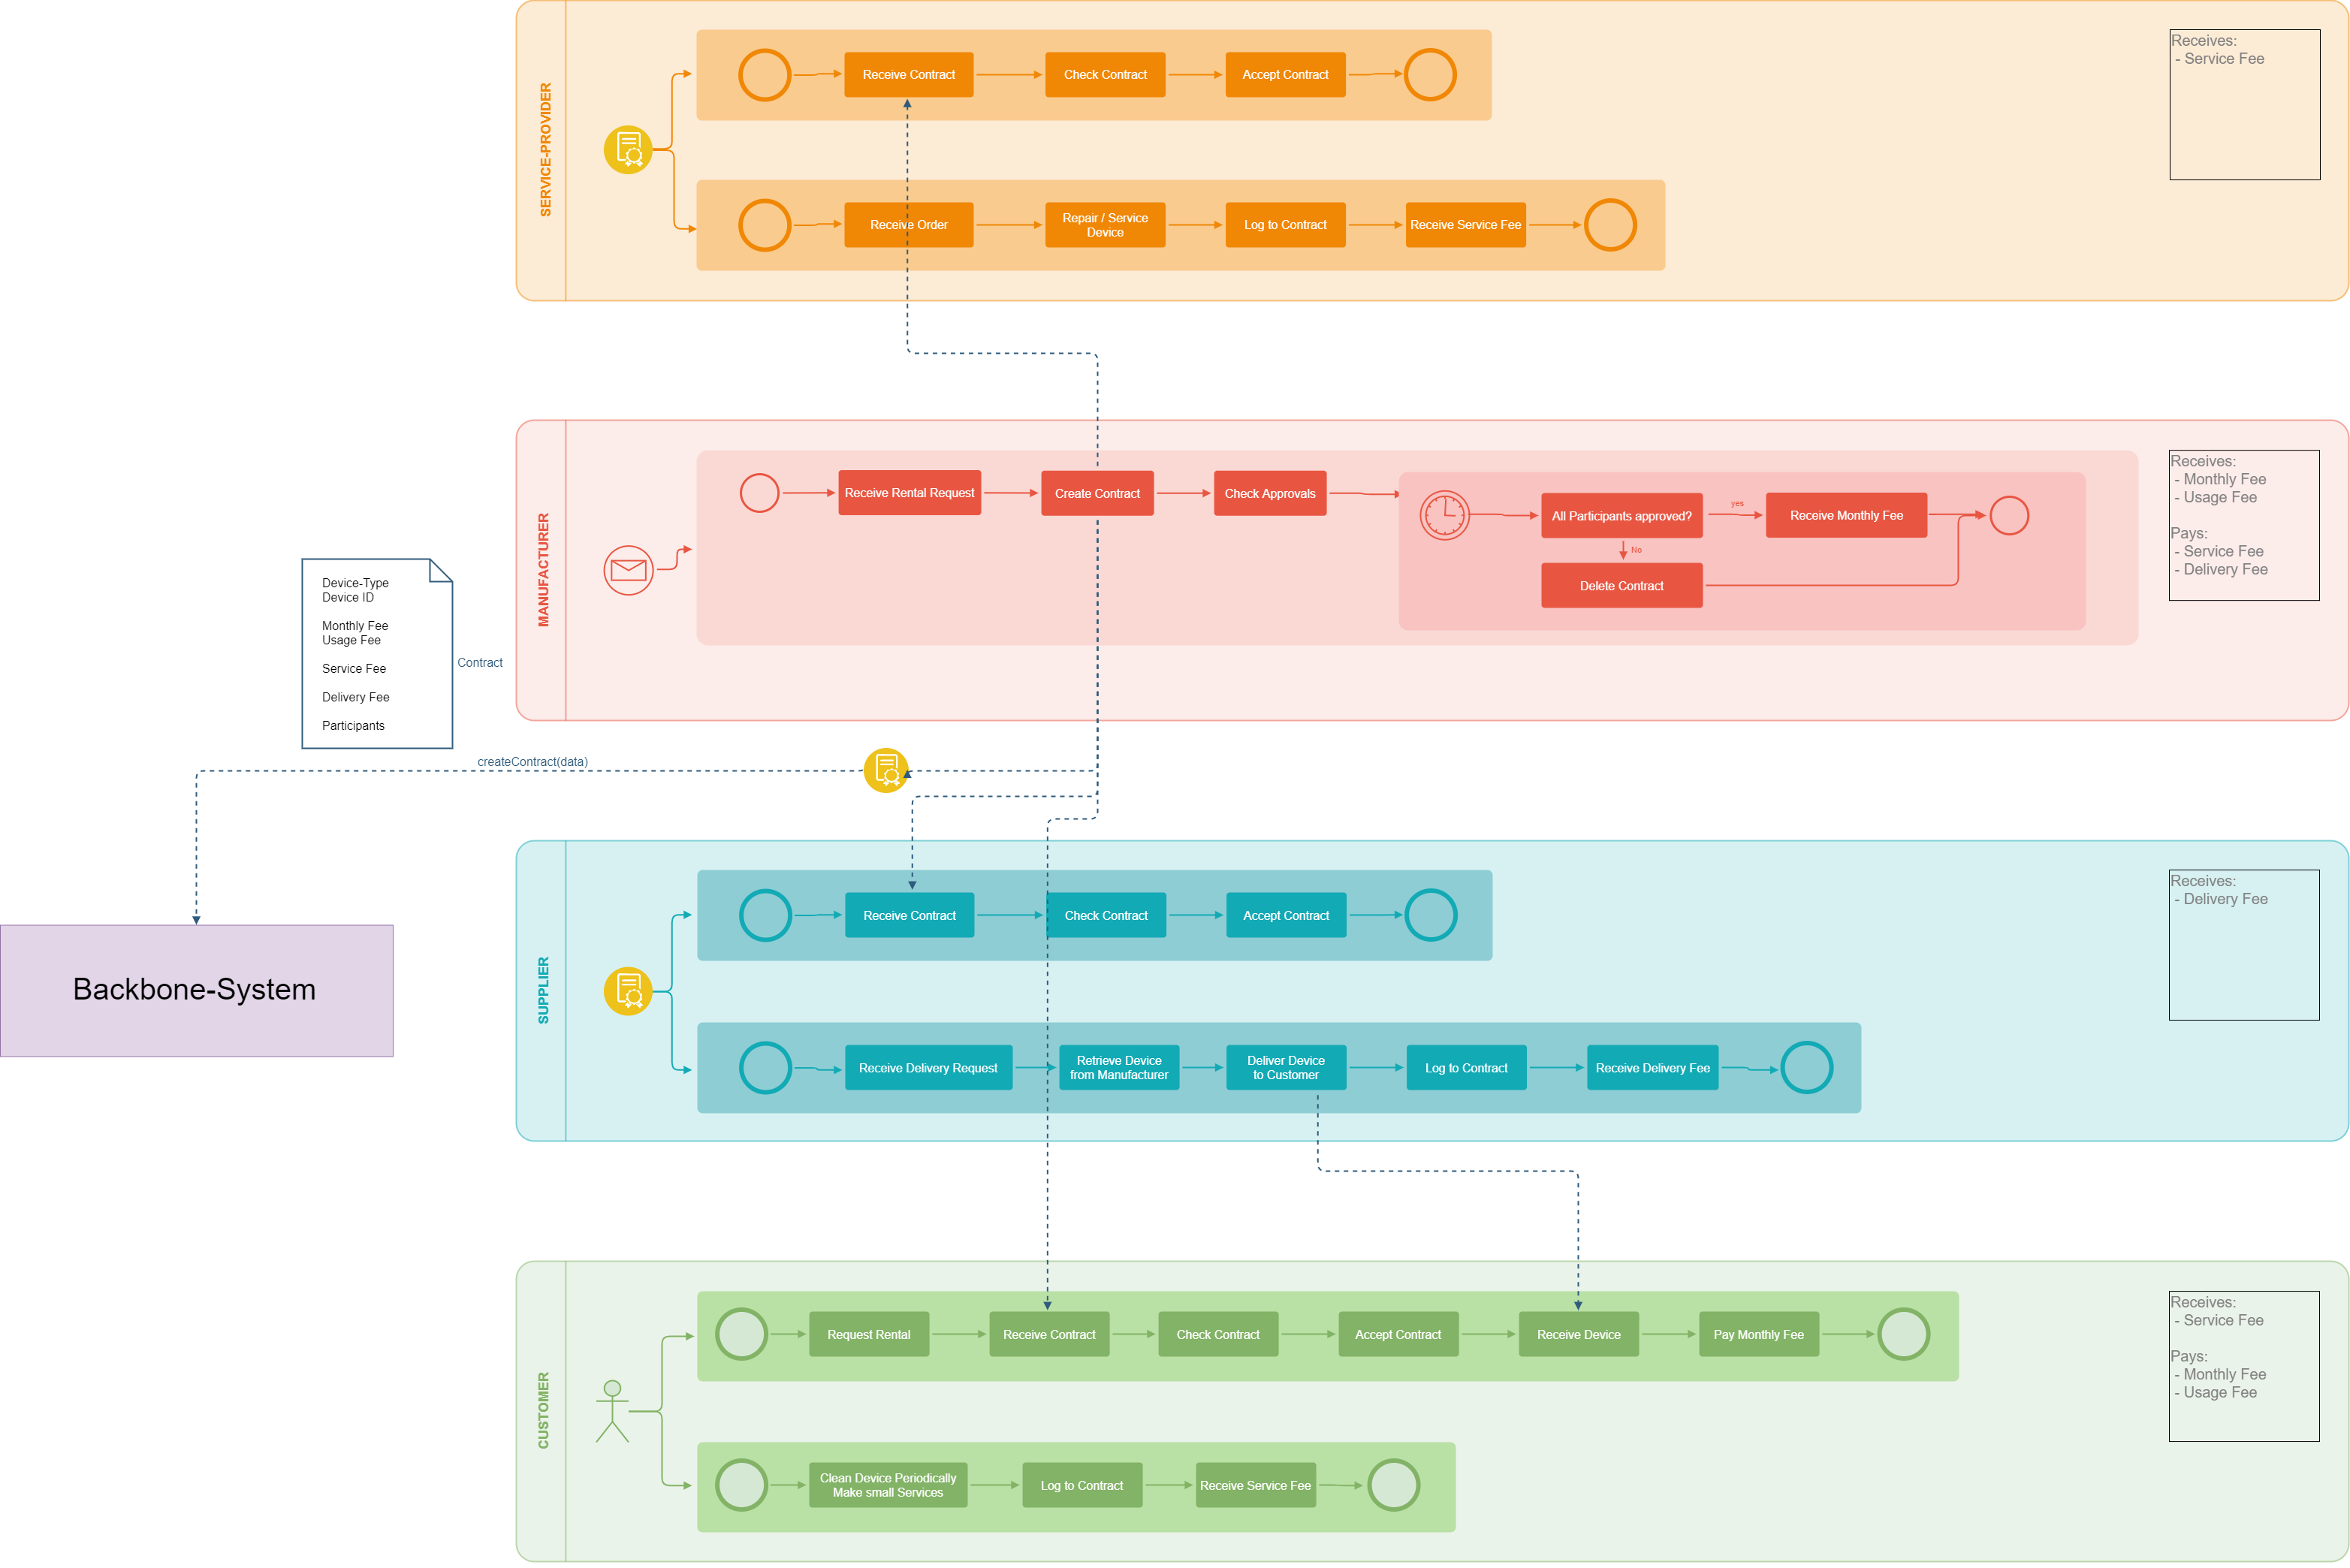
\includegraphics[width=1.0\textwidth]{gfx/IOT-Anwendungsfall_Ablauf.png}
 \caption{Grober Ablauf des Anwendungsfalls}
 \label{fig:chapter04:usecase_workflow}
\end{figure}

%
% Section: Technische Lösungsskizze
%
\section{Technische Lösungsskizze}
\label{sec:iot_usecase:solution}
In dieser Arbeit wird der oben beschriebenen Anwendungsfall basierend auf einer \ac{DLT}-Lösung prototypisch umgesetzt. Neben den beteiligten Stakeholdern besteht das Gesamtsystem aus einem Frontend, dass jedem Stakeholder die für ihn relevanten Funktionen zur Verfügung stellt und Informationen anzeigt. Das Backend des Systems besteht aus einer \ac{DLT}-Lösung\footnote{Die konkrete Implementierung, die als Backend-System eingesetzt wird, wird im Laufe dieser Arbeit ermittelt.}.

\subsection{Endgeräte}
\label{subsec:iot_usecase:solution:device}
Jedes Gerät besitzt eine eindeutige Identifikationsnummer und eine eindeutige Referenz zu dessen Eigentümer (Hersteller). Befindet sich ein Gerät in Vermietung, so existiert zwischen dem Mieter (Kunde) und dem Vermieter (Hersteller) ein Vertrag, der auf der Plattform persistiert wird. Das Gerät hat über das Internet Zugriff auf diese Plattform und damit auf den Vertrag, in dem wichtige Informationen zu den Rahmenbedingungen wie der Dauer des Vertragsverhältnisses oder die Kosten einer verbrauchten Einheit. Die Sensoren zum Registrieren des Verbrauchs und des Gerätestatus befinden sich auf dem Gerät selbst. Diese melden alle gesammelten Daten an eine Sammelstelle am Gerät. Dort werden die Daten aufbereitet, gemäß Vertrag verarbeitet und gesammelt. In einem regelmäßigen Intervall meldet das Gerät alle relevanten Daten wie Nutzung, Reinigungs- und Wartungsarbeiten und sonstige Informationen an das Backend und den verknüpften Vertrag, der wiederum die entsprechenden Geld-Transfers in die Wege leitet (siehe unten). In Abbildung \ref{fig:chapter04:usecase_device} wird ein Endgerät schematisch dargestellt.

\begin{figure}[htbp]
 \centering
 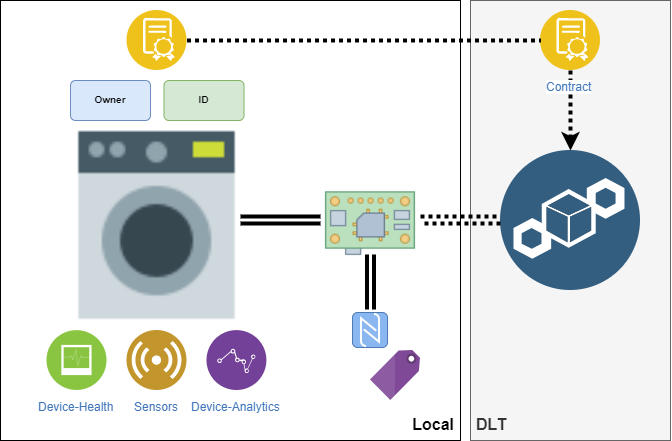
\includegraphics[width=1.0\textwidth]{gfx/IOT-Anwendungsfall_Device.png}
 \caption{Aufbau und Bestandteile eines Endgeräts}
 \label{fig:chapter04:usecase_device}
\end{figure}

\subsection{Verträge}
\label{subsec:iot_usecase:solution:contracts}
Verträge (Mietverträge, Service-Verträge, Lieferverträge) werden von allen beteiligten Parteien digital unterschrieben und im Backend gespeichert. Sie halten verschiedene Informationen, unter anderem über die Vertragslaufzeit, die Kosten sowie die zu erbringenden Leistungen der Parteien. Der Vertrag beinhaltet Mechanismen zur Begutschriftung und zur Belastung der Konten aller Beteiligten; die folgende Auflistung nennt alle wichtigen Geld-Transfers:
\begin{itemize}
  \item Nutzung durch den Kunden (Sender ist der Kunde, Empfänger ist der Hersteller)
  \item Reinigung durch den Kunden (Sender ist der Hersteller, Empfänger ist der Kunde)
  \item Wartung durch den Service-Dienstleister (Sender ist der Hersteller, Empfänger ist der der Service-Dienstleister)
  \item Lieferung durch den Lieferanten (Sender ist der Absender, Empfänger ist die Lieferant)
\end{itemize}

\subsection{Benutzerschnittstelle}
\label{subsec:iot_usecase:solution:frontend}
Das Frontend stellt eine grafische Benutzerschnittstelle bereit, die je nach Stakeholder die relevanten Informationen und Funktionalitäten bereitstellt. Um an der Plattform teilnehmen zu können, muss ein Registrierungsprozess durchlaufen werden und die Rolle bestimmt werden (Hersteller, Kunde, ...). Jeder Rolle ist der Zugriff auf eine Ansicht gestattet:
\begin{description}
  \item[Hersteller-Ansicht] Eine Übersicht über alle Geräte sowie deren Status, ob sie sich derzeit in Vermietung befinden, gibt dem Hersteller Aufschluss über die momentane Gesamtlage. Laufende Verträge können eingesehen und aktuelle Mietanfragen bearbeitet werden.
  \item[Kunden-Ansicht] Die gemieteten Geräte sowie die damit verbundenen, laufenden Verträge werden angezeigt. Es besteht Transparenz über Verbrauchs- und Statusinformationen, die die Geräte an die Plattform übermitteln. Laufende Kosten und aktueller Verbauch werden übersichtlich dargestellt. Es können Verträge gekündigt und neue Geräte gemietet werden.
  \item[Service-Dienstleister-Ansicht] Eine Übersicht über alle aktuell laufenden Service-Verträge wird angezeigt. Alle Meldungen über Service-Anfragen und Aufträge werden aufgelistet. Die Einnahmen durch Reparaturen und Services sowie den Kontostand werden detailliert dargestellt.
  \item[Lieferanten-Ansicht] Eine Übersicht über alle aktuell laufenden Lieferverträge wird angezeigt. Die Einnahmen durch Auslieferungen sowie den Kontostand werden detailliert dargestellt.
\end{description}

\subsection{Backend}
\label{subsec:iot_usecase:solution:backend}
Als dezentrale Plattform verwaltet und speichert das Backend alle Verträge sowie die Identitäten, Konten (Wallets) und Interaktionen der oben aufgelisteten Stakeholder. Die Implementierung auf einer \ac{DLT} kann in zwei verschiedenen Ausprägungen erfolgen, welche im Folgenden kurz dargelegt werden:\\
Die einfachste Lösung eine \ac{DLT} zur Versionierung und Speicherung von Daten einzusetzen entspricht einer simplen, dezentralen Hash-Datenbank. Hierbei wird der Status bestehend aus Mietverträgen, Kontoständen, Benutzerinteraktionen und Weiteren als Hashwert abgebildet und in der \ac{DLT} persistiert. Somit wird ein einfaches Logging ermöglicht; die Stärken einer \c{DLT} werden allerdings nicht eingesetzt. An dieser Stelle ergibt die Frage, welchen Vorteil die umfangreiche Konfiguration und Einrichtung einer \ac{DLT} im Vergleich zu einer klassischen verteilten Datenbank mit sich bringt.\\
Die zweite Variante setzt die Stärken einer \ac{DLT} geschickt ein und geht weit über das einfache Logging hinaus: Anstatt Hashwerte von einer Menge von Informationen zu bilden und diese in der \ac{DLT} zu speichern, werden die Informationen wie Benutzerinteraktionen, Miet- und Service-Verträge in die Blockchain geschrieben. Darüber hinaus geschieht die Vertragsabwicklung wie Zahlungstransaktionen, Vertragslogiken, etc. direkt auf der Blockchain und kann dort manipulationssicher verarbeitet werden. Zahlungen werden instantan ohne Integration eines Drittanbieters wie zum Beispiel PayPal oder Ähnliche abgewickelt und können nachvollziehbar und transparent persistiert werden. Zusammengefasst bedeutet das, dass die optimale Lösung dieses Anwendungsfalls auf Basis einer \ac{DLT} die Fähigkeiten dieser voll ausnutzt, indem Logging, Vertragsabwicklung, Payment und Manipulationssicherheit onchain ausgeführt werden.\\
Das Ziel der Umsetzung dieses Anwendungsfalls ist die Implementierung der zweiten Variante, um einen realistischen Anwendungsfall zielbringend zu implementieren und um einen entsprechenden Mehrwert durch den Einsatz einer \ac{DLT} zu generieren.
